% ------------ NEW CHAPTER ------------
\chapter{Technológie}   % TODO Zmenit nazov kapitoly, nie Zakladna terminologia
\label{chap:technologie}

V tejto kapitole sa zoznámime so základnymi pojmami, princípmi a spôsobmi, ktoré súvisia s probletikou tejto práce a ktoré budú ďalej využívané.
Kapitola opisuje základné rozdelenia zbraní do viacerých kategórií, princíp spracovania digitálneho obrazu.
Následne vysvetľuje z akým problémov pozostáva detekcia a rozpoznávanie objektov v obraze, opisuje populárne prístupy pre detekciu objektu.
A podrobne popisuje rôzne spôsoby pre klasifikáciu objektov do 2 alebo aj viacerých kategórií, ktoré sa v tejto práci budú používať.


\section{Zbrane}
\label{sec:weapons}
Obvyklá definícia hovorí, že zbraň je nástroj, predmet, či dokonca celé zariadenie,
ktoré je prispôsobené k~vyvolaniu zranenia na živý organizmus alebo k~ničeniu objektu \cite{book:StrelneZbrane}.
Za prvé zbrane môžeme považovať kopije, ktoré používali ľuďia pri love zvierat asi pred 400,000 rokmi \cite{prop:SpearHistory}.

Vo všeobecnosti môžeme zbrane rozdeliť podľa mnohých kritérií, napr. podľa zdroja energie použitej k~vypudeniu projektilu zo zbrane,
podľa konštrukcie a režimu streľby, ďalej z~hľadiska postupu pri nabíjaní alebo podľa veku zbrane, na nové - slúžiace svojmu účelu a historické - ktoré sú už nespôsobilé k~pôvodnemu účelu.
My sa zameriame na 2 základné rozdelenia a to poďla toho, ako zbrane pôsobia na živú silu, delíme na \cite{book:StrelneZbrane}:
\begin{enumerate}
	\item[$\bullet$] \textbf{Strelné} - rozrušujú vzdialený cieľ, živý alebo neživý, prodstredníctvom dopadovej energie strely vypudenej zo zbrane,
	\item[$\bullet$] \textbf{Chladné} - účinkujú bodom alebo sekom naostrenej čepele, ktorá je vsadená do rukoväťe alebo je nasadená na tyč či porísko,
    \item[$\bullet$] \textbf{Úderné} - pôsobia na živý objekt tupým úderom svojej časti, ktorá býva spojená s~vhodnou rukoväťou,
\end{enumerate}
a podľa ovládateľnosti a možnosti prenášania ich delíme na \cite{book:StrelneZbrane}:
\begin{enumerate}
	\item[$\bullet$] \textbf{Ručné} strelné zbrane môže prenášať a ovládať jediná osoba. Sú ovládané buď jednou rukou - krátke zbrane - alebo oboma rukami - dlhé zbrane,
	\item[$\bullet$] \textbf{Lafetované} zbrane musia byť vzhľadom ku svojej hmotnosti a rozmerom umiestnené na zvláštnom podstavci - \textit{lafete}. Takúto zbraň takisto väčšinou obsluhuje viac ľudí.
\end{enumerate}
V~tejto práci sa zameriame na strelné a ručné zbrane s~rozdelením na krátke a dlhé.



\section{Spracovanie obrazu}

Pre popis obrázkov a ostatných signálov sú často používané matematické modely.
Kde signál je funkcia závislá na určitých premenných s fyzikálnym významom, môže byť 1-dimenzionálna (napr. závisla na čase),
2-dimenzionálna (napr. obrázok závislý na 2 koordinátoch v ploche), 3-dimenzionálna (napr. popis pozície objektu v priestore), alebo aj viac-dimenzionálna \cite{book:ImageProcessing}.

    Každý obraz môže byť definovaný ako spojitá funkcia s dvomi neznámymi $f(x,y)$ kde $x$ a $y$ sú súradnice v ploche.
Tento spojitý obraz je digitalizovaný na tzv. vzorkovacích miestach.
Tieto vzorkovacie miesta sú usporiadané v ploche, ich geometrický vzťah sa nazýva mriežka.
Digitálny obraz je potom dátova štruktúra, ktorá je bežne reprezentovaná ako matica.
Jeden bod v mriežke reprezentuje jeden element 2-dimenzionálneho obrazu nazývany pixel, v 3-dimenzionálnom obraze sá tento element nazýva voxel \cite{book:ImageProcessing}.
Pri viac-dimenzionálnych digitálnych obrazoch sa pri spracovaní obrazu používa vektor hodnôt(napr. RGB hodnoty obrazového bodu).

Oblasť spracovania digitálneho obrazu je v dnešnej dobe veľmi široká a nachádza uplatnenie vo viacerých oboroch.
Môže sa využívať pri automatickej vizuálnej inšpekcií produktou, pre zaistenie vyššej produktivity a kvality výrobku v továrňach.
Ďalej pri spracovaní snímkov z lietadiel alebo satelitov pre získanie dát o prírodnych zdrojoch, ako napr. v poľnohospodárstve alebo lesníctve.
Širokú aplikáciu má v medicíne pri obrázkoch získavaných pomocou röngenových zariadení, CT a magnetickej rezonancie \cite{book:ImageProcessingApplication}.
A v súčastnosti taktiež v automobilovom priemysle pri rozvýjajúcej sa oblati autonómneho riadenia automobilov.



\section{Detekcia objektu v obraze}
\label{sec:detekcia}

V prvom rade je potrebné povedať že detekcia objektu a klasifikácia v obraze je veľmi dobre známy problém v oblasti spracovania obrazu.
V dnešnej dobe už niektoré modely prebehli svojou presnosťou a výkonom aj človeka \cite{prop:NNvsHuman}.

Rozoberaním problému lokalizácie a správnej klasifikácie objektu v obraze, skončíme s potrebou
    detekcie a klasifikácie niekoľkých objektov súčašne v jednej scéne.
Detekcia objektu v obraze je problém pozostavajúci z hľadania a klasifikovania variabilného počtu a rôznych typov objektov v obraze.
Dôležitým rozdielom je ``variabilná'' časť. V porovnaní s klasifikáciou je výstup detekcie objektov rôznorodý svojou dĺžkou, kedže
    počet objektov v obraze sa môže meniť z obrázka na obrázok \cite{odkaz:ObjectDetectionOverview}.

\subsection{Prehľad existujúcich riešení}

\subsubsection{Klasický prístup}
Aj keď v priebehu rokov bolo množstvo rôznych typov riešení, pre túto prácu je vhodné spomenúť 2 hlavné prístupy.

Prvý z nich je Viola-Jones spôsob, ktorý navrhol v roku 2001 Paul Viola a Michael Jones v práci \cite{prop:Viola2001RobustRF}.
Tento prístup je rýchly a relatívne jednoduchý, až natoľko že sa tento algoritmus implementuje v kamerách s bodovým snímačom, ktorý umožnuje
    detekciu tvári v reálnom caše s malým množstvom potrebného výkonu.
V jednoduchosti, algoritmus generuje rôzne, môže až tisíce, jednoduché binárne klasifikátory pomocou tzv. Haar funkcií.
Tieto klasifikátory sú kaskádovito zoradené a vyhodnocované v poradí podľa ich zložitosti, s využitím viacnásobneho posuvného okna [eng. multi-scale sliding window].
V prípade negatívnej klasifikácie v ktorejkoľvek úrovni vyhodnocovania, je tento proces ukončený a pokračuje sa klasifikáciou nad dalším podoknom [eng. subwindow] \cite{prop:Viola2001RobustRF}.

Druhý spôsob je klasifikácia pomocou histogramu orientovaných prechodov [eng. histogram of oriented gradients] a Support Vector Machine, ktorý bude podrobne
    rozobratý v kap. \ref{sec:klasifikacia}. Tento prístup takisto používa viacnásobne posuvné okno, avšak aj keď je lepší ako Viola-Jones, je oveľa pomalší \cite{odkaz:ObjectDetectionOverview}.

\subsubsection{Prístup pomocou hlbokých neurónovych sieti}
S prípochom neurónovych sieti prišla aj veľká zmena v oblasti spracovania obrazu, preto je vhodné spomenúť niekoľko spôsob
    detekcie objektov ktoré stavajú na neurónovych sieťach.

\textbf{R-CNN} je jeden z prvých riešení \cite{prop:rcnn}, v ktorom navrhovali 3 stupňový prístup:
\begin{enumerate}
	\item[$\bullet$] extrahovať možné objekty pomocou metódy regionálnych návrhov [eng. region proposal],
    \item[$\bullet$] extrahovať príznaky z každého regiónu pomocou konvolučnych neurónovych sieti,
    \item[$\bullet$] klasifikovať každý región pomocou Support Vector Machine.
\end{enumerate}

\textbf{Fast R-CNN} je označenie pre prístup ktorý vylepšil predchadzajúci R-CNN, základom je že stavia už iba na využítí konvolučnych neurónovych sieti.
V práci použili 2 prístupy k detekcii objektu, sliding window a region proposal.
Výsledky ukázali že prístup pomocou region proposal bol rýchlejší a dosiahli rýchlosť spracovania až 2 snímkov za sekundu \cite{prop:fast-rcnn}.
\begin{figure}[H]
    \centering
    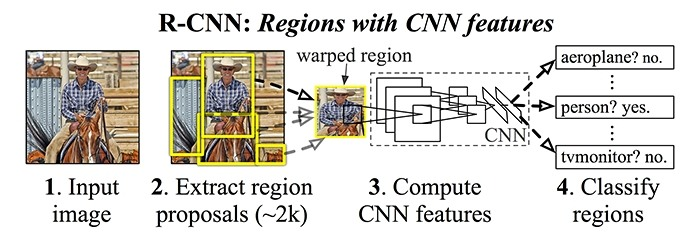
\includegraphics[width=0.8\textwidth]{rcnn}
    \qquad
    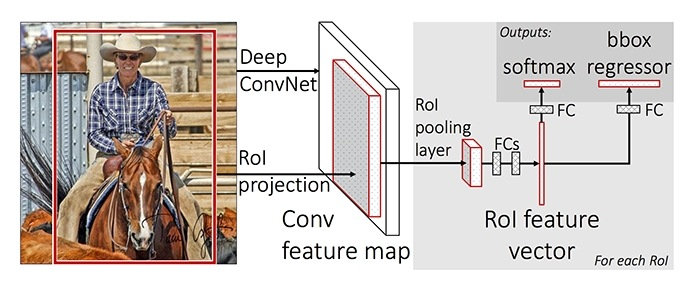
\includegraphics[width=0.6\textwidth]{fast-rcnn}
    \caption{Porovnanie architektúr R-CNN(hore) a Fast R-CNN(dole) \cite{odkaz:ObjectDetectionOverview}.}
    \label{pic:FastRCNN}
\end{figure}

\textbf{YOLO} [eng. You Only Look Once], rieši problem detekcie objektu v obraze ako regresívny problém.
Namiesto bežného postupu ako je najprv použitie region proposal techniky a následne klasifikovanie týchto regiónov.
To vedie YOLO k veľmi rýchlemu spracovaniu v reálnom čase ale za cenu presnosti.
Týmto spôsobom YOLO dokáže dosiahnuť 63.4\% mAP s 22 ms oneskorením \cite{prop:Redmon2016YouOL}.

\begin{comment}
    \subsubsection{Vyhľadávač na základe vizuálnej podobnosti obrázkov}
    Jednu z možných aplikácií detekcie objektov v obraze využíva Pinterest\footnote{\url{https://medium.com/@Pinterest_Engineering/introducing-automatic-object-detection-to-visual-search-e57c29191c30}}.
    Používaju detekciu objektov pre indexovanie rôznych častí obrázka.
    Týmto spôsobom si môže užívateľ pri hľadaní npr. špecifickej kabelky alebo topánok nájsť aj jej podobné.
    \begin{figure}[H]
        \centering
        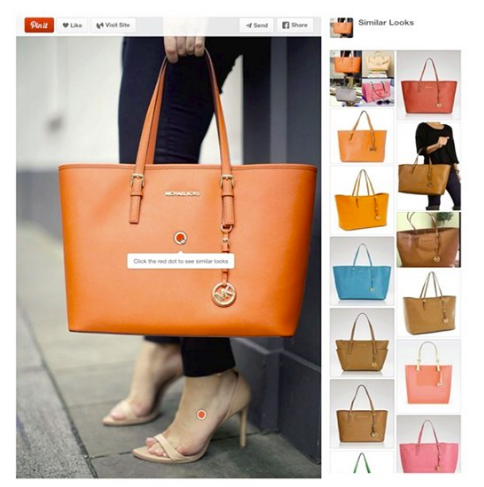
\includegraphics[width=0.5\textwidth]{purse}
        \caption{Prototyp automatického označovania a vyhľadávania objektov\cite{odkaz:ObjectDetectionOverview}}
        \label{pic:kNN}
    \end{figure}
\end{comment}

\subsection{Kĺzajúce okno}
\label{subsec:slidingwindow}
Kĺzajúce okno [eng. Sliding window] je jedná z metód pre detekciu objektov v obraze.
Táto metóda je veľmi vyčerpávajúca pretože zakladá na veľkom počte kandidátnych okien, až $10^4$, vo vstupnom obrázku.
Metóda prechádza vstupný obrázok na všetkých lokáciách s rôznou veľkosťou okna, následne na každom ``okne'' spúšta klasifikátor.
Nevýhodou tohto prístupu je jeho časová nárocnosť, preto sa tento spôsob nedá použiť pri spracovaní obrazu v reálnom čase.
Ale na druhú stranu metóda poskytuje dobrú presnosť pri kvalitnom klasifikátore \cite{prop:AutomaticHandgunDetection}.

\subsection{Regionálne návrhy}
\label{subsec:regionproposal}
Metóda regionálych návrhov [eng. region proposals] na rozdiel od metódy kĺzajuceho okna, nepredpokladá za kandidátne okná všetky možnosti.
Tieto kandidátne okná su vybrané pomocou metód návrhu detekcie [eng. detecion proposel methods], konkrétne metódy
    a ich porovnanie je môžné nájsť v članku \textit{What makes for effective detection proposals?} \cite{prop:ProposalMethods}.
Prvý model na detekciu objektov ktorý použit konvolučné neurónové siete s touto metódou pre výber okien bol R-CNN \cite{prop:AutomaticHandgunDetection}.



\section{Rozpoznávanie a klasifikácia}
\label{sec:klasifikacia}

Ako bolo spomenuté v úvode v kapitole \ref{sec:detekcia}, klasifikácie je jeden z aspektov pri detekcií a rozpoznávani objektov v obraze.
V tejto podkapitole bude podrobne popísaných niekoľko algoritmou pomocou ktorých je možné objekty z obrazu klasifikovať do kategórií.



\subsection{K-Nearest-Neighbor}
\textit{k}-Nearest Neighbor je algoritmus, ktorý sa učí pod dozorom [eng. supervised learning algorithm] často používaný pri rozpoznávaní vzorov v klasifikácií,
avšak je možné ho použiť aj pre odhad a predikciu \cite{book:DataMining}.
Algoritmus je pamäťovo náročný [eng. memory-based] a nepotrebuje žiaden trénovací model.
Pre jeho fungovanie nie je potrebný žiaden explicitný postup trénovania, okrem zberu vektorov príznakov s označeniami tried do ktorých patria.

Klasifikácia dát prebieha v 2 krokoch: nájdenie \textit{k} najbližších susedov spomedzi trénovaných dát a
vykonanie ''väčšinového hlasovania'' medzi nájdenými susedmi pre priradenie najčastejšie sa vykytovaného označenia triedy.

Nech $\{ (x_i, y_i); i = 1, 2, \dots, n \}$ je množína trénovacích dát, kde $x_i$ je vektor príznakov a $y_i$ je názov triedy do ktorej patrí vektor $x_i$.
Predpokladáme že každé $x_i$ je v určitom multidimenzionálnom priestore príznakov s metrikov $P$ a $y_i \in \{ 1, 2, \dots, l \}$, kde $y_i$ je číslo odpovedajúcej triedy.
Cieľom je priradiť neoznačeny vektor $x$ do zodpovedajucej triedy z množiny $\{ 1, 2, \dots, l \}$.

Najjednoduchšia verzia algoritmu \textit{k}-NN je 1-NN, kde vektor $x$ je priradený najbližsiemu susedovi.
To znamená že ak $x_j$, kde $j \in \{ 1, 2, \dots, n \}$, je najbližšií k $x$ vo forme vzdialenosti $P$ \cite{prop:KnnClassification}:
\begin{equation}
    \label{eq:kNNMetric}
    x_j = arg \; min_{\{x_i, 1 \leq i \leq n\}} P(x, x_i)
\end{equation}
tak označenie triedy pre vektor $x$ je číslo $y_i$.

Pre formu algoritmu \textit{k}-NN, kde $k > 1$ je postup podobný, ale priradenie označenia triedy pre $x$ je na základe najčastejšie sa vyskytovaného označenia triedy
spomedzi \textit{k} najbližších susedov z trénovacích bodov $x_i$, kde $k$ je užívateľom definovaná konštanta \cite{prop:KnnClassification}.

Najbežnejší výpočet pre vzdielenosť bodov je pomocou Euklidovskej vzdielenosti.
Táto vzdielnosť $d_{a,b}$ je medzi dvoma $J$-dimenzionálnymi vektormi $a$ a $b$ vyjadrená ako \cite{prop:KnnClassification}:
\begin{equation}
    \label{eq:euclidMetric}
    d_{a,b} = \sqrt{\sum_{j=1}^{J}{(a_j - b_j)^2}}
\end{equation}

Na obrázku \ref{pic:kNN} je zobrazený rozdiel medzi 1-NN a 5-NN algoritmom pre klasifikáciou,
    použitím 2-dimenzionálnych bodov a 3 tried dát (červená, modrá, zelená).
Farebné regióny vyznačujú rozhodovacie hranice klasifikátora, ktorý využíva Euklidovskú vzdielnosť.
Biele oblasti ukazujú body, ktoré sú nejednoznačne klasifikované (to znamená, že hodnotenie triedy je viazané aspoň na dve triedy).
V ukážke je vidno že v prípade 1-NN klasifikátora, niektré body vytvárajú ''malé ostrovy''
    (napr. zelený bod v strede mraku medzi modrými bodmi), zatiaľ čo 5-NN klasifikátor vyhladzuje tieto nezrovnalosti,
    a pravdepodobne vedie k lepšiemu zovšeobecneniu nad testovacími údajmi.

\begin{figure}[H]
	\centering
	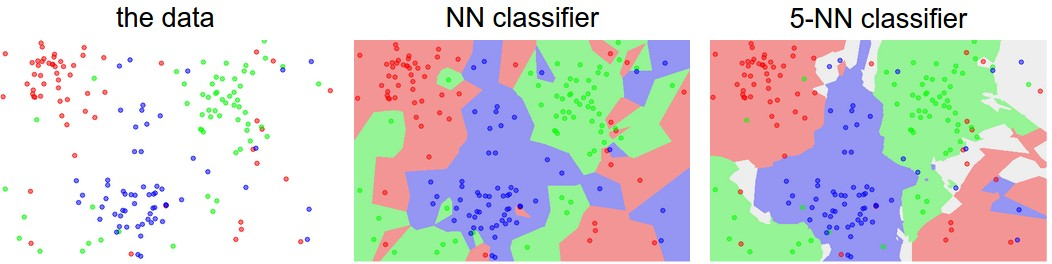
\includegraphics[width=1\textwidth]{knn}
	\caption{Porovnanie k-NN klasifikátorov \cite{odkaz:KnnImage}.}
	\label{pic:kNN}
\end{figure}



\subsection{Support Vector Machines}
Support Vector Machines (SVM's) sú metódy učenia používané pre binárnu klasifikáciu.
Základnou myšlienkou je nájdenie hyper--roviny, ktorá perfektne oddelí \textit{d}--dimenzionálne dáta do dvoch tried \cite{prop:IntroductionToSVM}.
SVM sa snaží maximalizovať vzdialenosť medzi rozdeľujúcou rovinou a dátami nachádzajúcimi sa v každej z 2 polrovín \cite{prop:SupervisedMachineLearning}.
Avšak kedže vstupné dáta väčšinou nie su lineárne separovatelné, SVM's predstavujú pojem “kernel induced feature space”,
    ktorý prevádza dáta do vyššieho dimenzionálneho priestoru, kde sú dáta oddeliteľné.\cite{prop:IntroductionToSVM}.

Ak trénovacie dáta sú lineárne separovatelné, tak dvojica $(w, b)$, kde $w$ je váhový vektor a $b$ je predpoveď
    (alebo $-b$ je prahová hodnota) existuje ako \cite{prop:SupervisedMachineLearning}:
\begin{equation}
    \label{eq:SVMPair1}
    w^T * x_i + b \geq 1, \; pre \; x_i \in P
\end{equation}
\begin{equation}
    \label{eq:SVMPair2}
    w^T * x_i + b \leq -1, \; pre \; x_i \in N
\end{equation}
s rozhodovacím pravidlom
\begin{equation}
    \label{eq:SVMDecisionRule}
    f_{w,b}(x) = sgn(w^T x + b)
\end{equation}
V tomto prípade keď je možné lineárne rozdeliť dve triedy, tak optimálna hyper--rovina pre rozdelenie
    môže byť nájdena, minimalizáciou kvadratickej formy rozdeľujúcej hyper--roviny
\begin{equation}
    \label{eq:SVMDecisionRule}
    mininimize_{w,h} \; \Phi(w) = \frac{1}{2}||w||^2, \; pre \; y_i(w^Tx_i + b) \geq 1, i = 1, \dots, l
\end{equation}

V tomto prípade lineárneho rozdelenia dát, pri nájdení optimálnej rozdeľujúcej hyper--roviny, dátove body, ktoré ležia na jej okraji
    sa nazývajú podporné vektorové body[eng. support vector points] a riešenie je reprezentované ako lineárna kombinácia iba 3 týchto bodov (vid. obrázok \ref{pic:SVMMAxMargin} ).
Ostatné body sú ignorované \cite{prop:SupervisedMachineLearning}.

\begin{figure}[H]
	\centering
	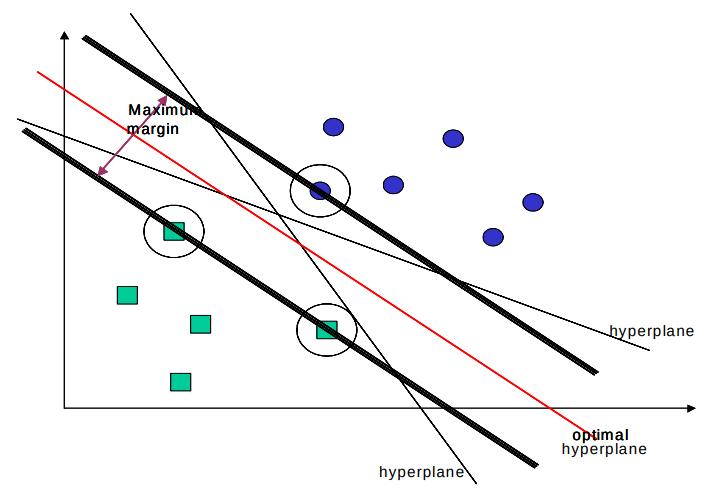
\includegraphics[width=0.8\textwidth]{SVM_max_margin}
	\caption{Maximálne rozpätie \cite{prop:SupervisedMachineLearning}.}
	\label{pic:SVMMAxMargin}
\end{figure}

Avšak väčsina reálnych problémou zahŕňa nelineárne rozdelenie dát pre ktoré neexistuje žiadna hyper--rovina, ktorá by úspešne rozdelila trénovacie dáta.
Riešenie tohto problému je mapovať dáta do vyššie--dimenzionálneho priestoru a definovať tam rozdeľujúcu hyper--rovinu.
Tento vyššíe-dimenzionálny priestor je tzv. transformovaný priestor príznakov[eng. transformed feature space], ako opak ku vstupnému priestoru[eng. input space] obsahujúcemu trénovacie dáta\cite{prop:SupervisedMachineLearning}.

Pri vhodne zvolenom transformovanom priestore príznakov dostatočnej veľkosti, môžu byť všetky trénovacie dáta rozdelitelné.
Lineárne rozdelenie v tomto priestore zodpovedá nelineárnemu rozdeleniu v pôvodnom vstupnom priestore.

Pri mapovaní dát do určitého Hilbertovho priestora \cite{prop:HilbertSpace} $H$ ako $\Phi:R^d \rightarrow H$.
Potom trénovací algoritmus závisý len na údajoch zo skalárneho súčinu[eng. dot products] v priestore $H$, t.j na funkciách v tvare $\Phi(x_i) * \Phi(x_j)$.
Ak bude existovať ''funkcia jadra''[eng. kernel function] $K$ ako $K(x_i, x_j) = \Phi(x_i)*\Phi(x_j)$, tak budeme musieť použiť iba funkciu $K$ v trénovacom algoritme
    a nikdy nebudeme potrebovať explicitne definovať $\Phi$ \cite{prop:SupervisedMachineLearning}.

Takže jadrá[eng. kernels] sú špeciálnou triedou funkcií, ktoré dovoľujú, aby sa vnútorné produkty vypočítali priamo vo funkčnom priestore[eng. feature space] bez toho, aby sa vykonalo vyššie popísané mapovanie.
Po vytvorení hyper--roviny sa funkcia jadra použije na mapovanie nových bodov do funkčného priestoru pre klasifikáciu \cite{prop:SupervisedMachineLearning}.

Voľba správnej funkcie jadra je veľmi dôležitá, kedže definujú transformovaný priestor príznakov v ktorom budú trénovacie dáta klasifikované.
Genton \cite{prop:KernelClasses} popísal niekoľko tried jadier, avšak, neadresoval otázku, ktorá trieda je najvhodnejšie pre daný problém.

\begin{comment}
    Zoznam populárnych jadier\cite{prop:SupervisedMachineLearning}:
    \begin{equation}
        K(x, y) = (x*y+1)^P
    \end{equation}
    \begin{equation}
        K(x, y) = e^{\frac{-||x-y||^2}{2 \sigma^2}}
    \end{equation}
    \begin{equation}
        K(x, y) = tanh(\kappa x*y - \delta)^P
    \end{equation}
\end{comment}


\begin{figure}[H]
	\centering
	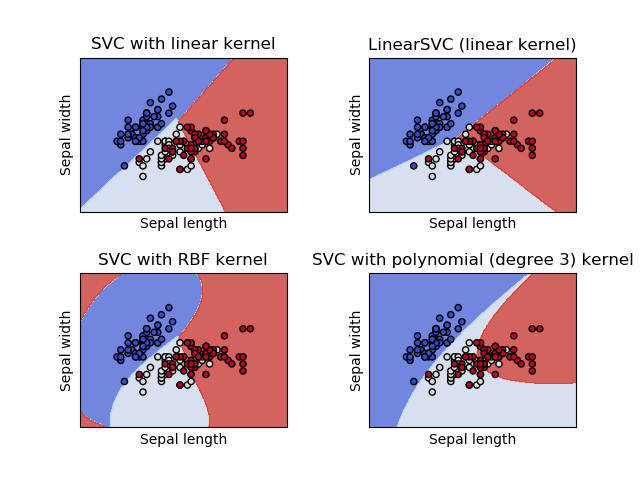
\includegraphics[width=1\textwidth]{sphx_glr_plot_iris_0012}
	\caption{Porovnanie SVM klasifikátora s použitím rôznym jadier \cite{odkaz:SVMImage}.}
	\label{pic:SVMComparison}
\end{figure}



\begin{comment}
\subsection{Stochastic Gradient Descent}
Výpočtova zložitosť algoritmov učenia sa stáva kritickým obmedzujúcim faktorom, pri používaní veľmi rozsiahlých množín vstupným dát.
Preto sa pre veľké množiny dát začal používať Stochastic Gradient Descent\cite{prop:StochasticGradientDescent}, ktorý tieto výpočty dokáže optimalizovať.

Každý vzor $z$ je pár $(x, y)$ kde $x$ je ľubovolný vstup a $y$ skalárny výstup.
Máme stratovú funkciu [eng. loss function] $\ell(\hat{y},y)$ ktorá meria hodnotu predpovedania $\hat{y}$ keď správna odpoveď je $y$,
    a zvolíme si rodinu $\mathcal{F}$ funkcií $f_w(x)$ parametrizované váhovym vektorom $w$.

Hľadáme funkciue $f \in \mathcal{F}$, ktorá minimalizuje stratu $Q(z,w) = \ell(f_w(x), y)$ spriemerovanú vzhľaďom na vzory $z$.
Avšak pre napodobenie prírody je prirodzenejšie priemerovať vzhľadom na neznámu distribúciu $dP(z)$\cite{prop:StochasticGradientDescent}.
\begin{equation}
    E(f) = \int{\ell(f(x), y)dP(z)} \quad E_n(f) = \frac{1}{n}\sum_{i=1}^{n}\ell(f(x_i), y_i)
\end{equation}
$E_n(f)$ meria výkonnosť trénovacích dát. $E(f)$ meria generalizovanú výkonnosť, teda očakávaný výkon v budúcich vzorkách.

Pomocou klesania gradientu[eng. gradient descent] minimalizujeme $E_n(f_w)$, kde každá iterácia aktualizuje váhove vektory $w$ na základne gradientu.
\begin{equation}
    w_{t+1} = w_t - \gamma \frac{1}{n}\sum_{i=1}^{n}\bigtriangledown_w Q(z_i, w_t)
\end{equation}
kde $\gamma$ je vhodne zvolený zisk[eng. gain].

Stochastic Gradient Descent algoritmus je drastické zjednodušenie.
Namiesto počítania gradientu pre $E_n(f_n)$, každá iterácia odhadne tento gradient na základe jednej náhodne vybranej vzorky $z_t$\cite{prop:StochasticGradientDescent}:
\begin{equation}
    w_{t+1} = w_t - \gamma \bigtriangledown_w Q(z_t, w_t)
\end{equation}
\end{comment}



\subsection{Neurónové siete}
\label{subsec:neuralnetworks}
Neurónová sieť [eng. neural network] (NN) je masívne paralelný procesor, ktorý má sklon k uchovávaniu experimentálnych znalostí a ich ďalšieho využívania.
Napodobňuje ľudský mozog v dvoch aspektoch \cite{odkaz:NNIntroduction}:
\begin{enumerate}
	\item[$\bullet$] poznatky sú zbierané v neurónovej sieti počas učenia,
	\item[$\bullet$] medzineurónové spojenia (synaptické váhy - SV) sú využívané na ukladanie znalostí.
\end{enumerate}
Toto je jedna z definícii neurónových sieti, akceptovaná komunitou.
Je zrejmé, že inšpirácia ku vzniku NN prišla z biologických systémov.
Na prvý dojem vysoko abstraktná disciplína nachádza množstvo aplikácii v praxi a stáva sa prostriedkom pre riešenie problémou v širokom spektre odborných oblastí \cite{odkaz:NNIntroduction}.

Rôzne architektúry umelých neurónových sieti[eng. artificial neural network] sa používajú pre riešenie rôznych úloh.
Konvolučné a rekurentné NN sú dve z najúspešnejších a sú z veľkej časti zodpovedné za nedávnu revolúciu umelej inteligencie \cite{odkaz:CorrectionOfImageOrentation}.

Vo všeobecnosti môžeme vymenovať nasledovné oblasti využitia neurónových sieti \cite{odkaz:NNIntroduction}:
\begin{enumerate}
    \item[$\bullet$] klasifikácie do tried, klasifikácia situácií,
    \item[$\bullet$] riešenie predikčných problémou,
    \item[$\bullet$] problémy riadenia procesov,
    \item[$\bullet$] tranformácia signálov.
\end{enumerate}

Neurónové siete sú usporiadané do vnútorne prepojených vrstiev umelých neurónov.
Jednoducho povedané, každá vrstva berie výstup z prechádzajucej vrstvy, aplikuje transformácie a výsledok pošle na vstup ďalšej vrstve.
Prvá vrstva vstupov je prepojená na vstupné dáta, ktoré sa majú spracovať a posledná vrstva je akýkoľvek výstup, ktorý chceme predpovedať \cite{odkaz:CorrectionOfImageOrentation} (vid. obrázok \ref{pic:NNExample}).
\begin{figure}[H]
	\centering
	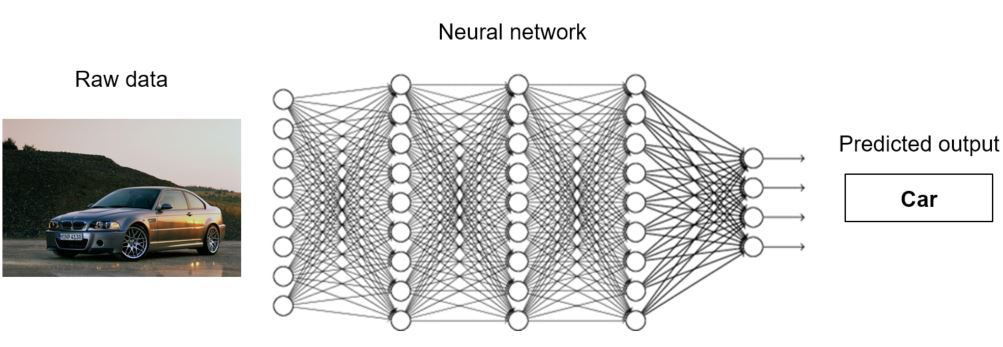
\includegraphics[width=1\textwidth]{nn}
	\caption{Jednoduchá architektúra NN s 1 vstupnou, 3 skrytími a 1 výstupou vrstvou \cite{odkaz:CorrectionOfImageOrentation}.}
	\label{pic:NNExample}
\end{figure}

\subsubsection{Perceptron}
Pre pochopenie fungovania neurónovej siete je potrebné najprv pochopiť umelý neurón, zvaný perceptron.
Perceptron vynašiel vedec Frank Rosenblatt v 1950 až 1960 roku, inšpirovaný predchádzajucov prácov Warren McCulloch a Walter Pitts.
Dnes sa bežné používa iný model umelého neurónu tzv. sigmoid neurón \cite{odkaz:HandwrittenDigitRecognision}.

V jednoduchosti, perceptron zoberie niekoľko vstupov, $x_1, x_2, \dots$ a reprodukuje ich na jediný binárny výstup.
\begin{figure}[H]
	\centering
	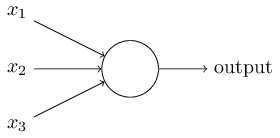
\includegraphics[width=0.4\textwidth]{tikz0}
	\caption{Jednoduchý príklad perceptronu \cite{odkaz:HandwrittenDigitRecognision}.}
	\label{pic:Perceptron}
\end{figure}
Rosenblatt navrhol jednoduché pravidlo pre výpočet výstupu.
Zaviedol váhy[eng. weights], $w_1, w_2, \dots$,
    reálne čisla ktoré vyjadrujú dôležitosť príslušných vstupov vzhľadom na výstupy.
Výstup neurónu, 0 alebo 1, sa určuje podľa toho či vážena suma $\sum_j w_j x_j$ je menšia alebo väčsia ako určitá prahová hodnota.
Matematické vyjadrenie aktivačnej funkcie perceptronu by potom bolo \cite{odkaz:HandwrittenDigitRecognision}:
\begin{equation}
    output = 0, \; ak \; \sum_j w_j x_j \leq threshold
\end{equation}
\begin{equation}
    output = 1, \; ak \; \sum_j w_j x_j > threshold
\end{equation}

Matematický model perceptronu je možné zjednodušiť a to prepísaním formuly $\sum_j w_j x_j$ na skalárny súčin[eng. dot product],
    $w*x \equiv \sum_j w_j x_j$, kde $w$ a $x$ sú vektory váh a vstupov.
Druhá zmena je presun prahovej hodnoty na opačnú stranu nerovnice, a nahradiť ju tzv. perceptron bias, $b \equiv -threshold$.
Použitím týchto úprav bude model vyzerať nasledovne \cite{odkaz:HandwrittenDigitRecognision}:
\begin{equation}
    output = 0, \; ak \; w*x + b \leq 0
\end{equation}
\begin{equation}
    output = 1, \; ak \; w*x + b > 0
\end{equation}

\begin{figure}[H]
    \centering
    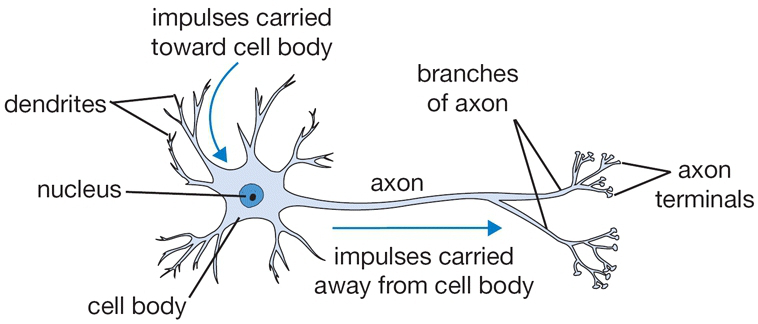
\includegraphics[width=0.5\textwidth]{neuron}
    \qquad
    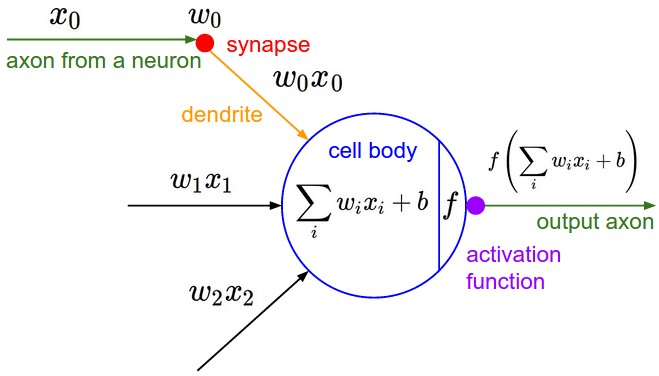
\includegraphics[width=0.4\textwidth]{neuron_model}
    \caption{biologický neurón(vľavo) a jeho matematický model(vpravo) \cite{odkaz:ConvolutionalNeuralNetworkCS231n}.}
    \label{pic:Neuron}
\end{figure}

\subsubsection{Sigmoid}
Sigmoid je jedna z aktivačných funkcií používana v neurónových sietach, jej matematická formula je
\begin{equation}
    \sigma(x) = \frac{1}{1 + e^{-x}}
\end{equation}
zobrazená na obrázku \ref{pic:ActivationFunctions} vľavo.

Funkcia zoberie skutočné číslo a ''stlačí'' ho do rozmedzia 0 až 1.
Kde veľké záporne čísla nadobudnú hodnotu 0 a veľke kladné čísla hodnotu 1.
Funkcia sigmoid sa historicky často používala pretože má peknú interpretáciu pre spúštanie ''výstrelu'' neurónu,
    od nevýpalanie (0) až po úplne nasýtenie strely pri predpokladanej maximálnej frekvancií (1).
V praxi, sa sigmoid používa už len zriedka.
Pretože ma 2 hlavné nevýhody \cite{odkaz:ConvolutionalNeuralNetworkCS231n}.
\begin{enumerate}
    \item[$\bullet$] \textbf{Zabíjanie prechodov [eng. gradients]} - keď sa aktivácia neurónu nasýti na obidvoch koncoch 0 alebo 1, gradient v týchto oblastiach je takmer nulový.
    Tento gradient sa používa pri spätnej propagácií [eng. backpropagation] v neurónových sietach. Preto ak je miestny gradient veľmi malý, takmer žiaden signál
    neurónom nepreteká k jeho váham a rekurzívne k jeho dátam. Rovnako ak pri inicializácií sú váhy príliš veľké, väčsina neurónov by bola nasýtených a sieť by sa sotva niečo učila.
    \item[$\bullet$] \textbf{Výstupy nie sú centrované na nulu} - to má dôsledky na dynamiku pri klesaní gradient-u, pretože ak sú údaje prichádzajúce do neurónu vždy kladné,
    potom gradient na váhach $w$ nadobudne, počas spätnej propagáciie, všetky hodnoty pozitívne alebo negatívne (v závisloti na gradient-e celého výrazu).
    To by mohlo viesť k nežiadúcej cik-cakovitej dynamike pri aktualizáciach gradient-ov pre váhy.
\end{enumerate}


\subsubsection{Tanh}
Funkcia tanh je dalšou z aktivačných funkcií neurónu je zobrazená na obrázku \ref{pic:ActivationFunctions} vpravo.
Tanh zoberie skutočné čislo a stlačí ho do rozmedzia -1 až 1. Pracuje podobne ako sigmoid.
Matematický zápis je \cite{odkaz:ConvolutionalNeuralNetworkCS231n}:
\begin{equation}
    tanh(x) = 2\sigma(2x) - 1
\end{equation}
Kedže netrpí nevýhodami ako sigmoid tak v praxi je preferovanejší.


\begin{figure}[H]
    \centering
    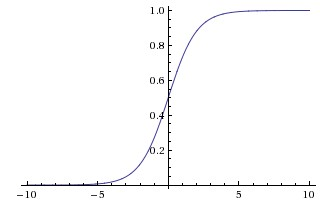
\includegraphics[width=0.45\textwidth]{sigmoid}
    \qquad
    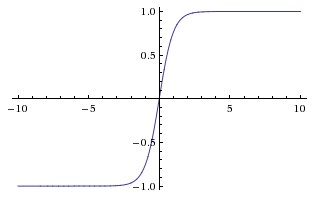
\includegraphics[width=0.45\textwidth]{tanh}
    \caption{
        Vľavo: Sigmoid nelineárne stlačenie čísel do rozsahu [0,1],
        Vpravo: Tanh nelineárne stlačenie čísel do rozsahu [-1,1] \cite{odkaz:ConvolutionalNeuralNetworkCS231n}.
    }
    \label{pic:ActivationFunctions}
\end{figure}

\subsubsection{ReLU a Leaky ReLU}
V praxi existuje niekoľko dalšich aktivačných funkcií, každá je použitelná pre riešenie iného problému,
    čiže každá ma svoje výhody ale aj nevýhody.
Ako príklad môžeme uviesť ReLU (Rectified Linear Unit)
\begin{equation}
    f(x) = max(0,x)
\end{equation}
alebo jeho obdobu Leaky ReLU, ktorá sa snaží vyriešiť nevýhody ReLU.
\begin{equation}
    f(x) = x \quad ak \; x > 0
\end{equation}
\begin{equation}
    f(x) = ax \quad ak \; x <= 0
\end{equation}
kde $a$ je malá konštanta (napr. 0.01) \cite{odkaz:ConvolutionalNeuralNetworkCS231n}.

\subsubsection{Architektúra neurónovej siete}
Ako bolo spomínane už vyššie, neurónová sieť je modelovaná ako kolekcia neurónov, ktoré sú prepojené v acyklickom grafe.
Modely neurónových sieti sú často organizované do odlišných vrstiev neurónov.
Pre bežné neurónové siete je najbežnejšou vrstvou tzv. plne-prepojená vrstva [eng. fully-connected layer],
    v ktorej sú neuróny medzi dvoma priľahlými vrstvami plne párovo prepojené, ale neuróny v jeden vrstve nemajú medzi sebou žiadne spojenia.
Na obrázku \ref{pic:NeuralNetworkArchitecture} nižšie sú uvedené dve topológie ktoré využívajú plne-prepojené vrstvy \cite{odkaz:ConvolutionalNeuralNetworkCS231n}:
\begin{figure}[H]
    \centering
    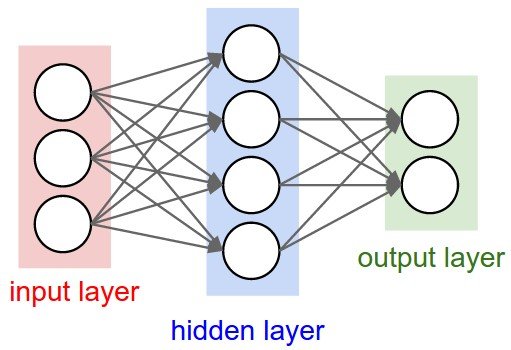
\includegraphics[width=0.38\textwidth]{neural_net}
    \qquad
    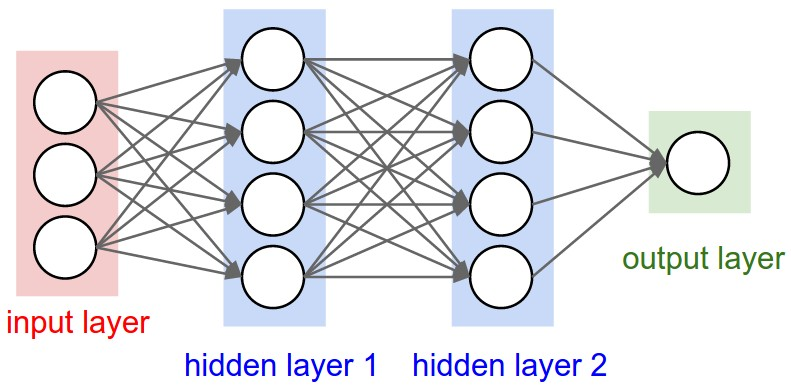
\includegraphics[width=0.52\textwidth]{neural_net2}
    \caption{Vľavo: 2-vrstvová neurónová sieť, Vpravo: 3-vrstvová neurónová sieť \cite{odkaz:ConvolutionalNeuralNetworkCS231n}.}
    \label{pic:NeuralNetworkArchitecture}
\end{figure}

Vačšie neurónové sieťe dokážu reprezentovať komplikovanejšie funkcie.
Na obrázku \ref{pic:XNNLayerExample} je vidieť rozdiel klasifikácie dát do 2 tried (červená, zelená) použitím rôzneho počtu vrstiev v neurónovej sieti.
\begin{figure}[H]
	\centering
	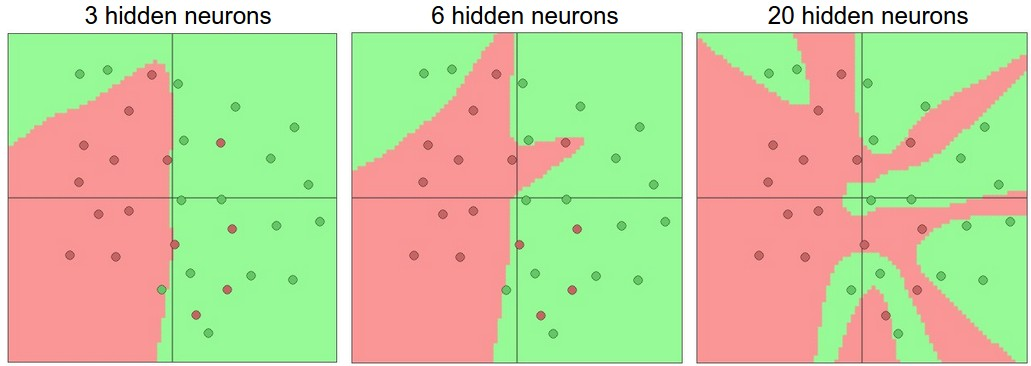
\includegraphics[width=1\textwidth]{layer_sizes}
	\caption{Zobrazenie klasifikácie dát rôzne veľkými neurónovými sieťami \cite{odkaz:ConvolutionalNeuralNetworkCS231n}.}
	\label{pic:XNNLayerExample}
\end{figure}

\subsection{Konvolučné neurónové siete}
\label{subsec:convolutionalneuralnetwork}
Konvolučné neurónové siete [eng. convolutional neural networks] (CNNs), sú špeciálnym prípadom neurónových sieti pre spracovanie
    dát, ktoré majú známu topológiu podobnú mriežke.
Pre príklad je možné uviesť 2-dimenzionálne dáta ako sieť pixelov pri spracovaní obrázkov.
Názov týchto sieti \textit{konvolučné} indikuje používanie matematickej operácie zvanej konvolúcia [eng. convolution] \cite{book:Goodfellow-et-al-2016}.

\subsubsection{Konvolúcia}
Vo svojej najvšeobecnejšej podobe, konvolúcia je operácia dvoch funkcií s reálnymi hodnotami argumentov.
Operácia konvolúcie je typicky označovaná hviezdičkou:
\begin{equation}
    s(t) = (x * w)(t)
\end{equation}
V terminilógií konvolučnej siete sa prvý argument (v tomto príklade funkcie $x$) často označuje ako vstup a druhý
    argument (v tomto príklade funkcia $w$) ako jadro [eng. kernel]. Výstup je niekedy označovaný ako mapa príznakov.

Bežne konvolúciu používame na viac ako jednej osy súčasne.
Pri použítí 2-dimenzionálneho obrázku $I$ ako náš vstup, budeme chcieť použiť aj 2-dimenzionálne jadro $K$ \cite{book:Goodfellow-et-al-2016}:
\begin{equation}
    S(i,j) = (I * K)(i, j) = \sum_m \sum_n I(m,n) K(i - m, j - n)
\end{equation}

Avšak množstvo knižníc, ktoré implementujú neurónové siete, používajú tzv. cross-correlation funkciu \cite{book:Goodfellow-et-al-2016}:
\begin{equation}
    S(i,j) = (I * K)(i, j) = \sum_m \sum_n I(i + m, i + n) K(m, n)
\end{equation}

Kde hlavným cieľom konvolúcie v konvolučných neurónových sietach je extrakcia príznakov zo vstupného obrázku.
V jednoduchosti je možné si predstaviť 2-dimenzionálne dáta (obrázok) o rozmeroch 5x5 pixelov, ktorých hodnoty sú 0 alebo 1.
Jadro alebo môžeme nazvať aj filter o veľkosti npr. 3x3, prechádza postupne celý vstupný obrázok s krokom 1 a ráta hodnotu výstupneho pixelu na základe svojich hodnôt ktoré obsahuje.
Výsledokom je potom mapa príznakov [eng. Feature map] označovaná aj ako aktivačná mapa [eng. Activation map] o veľkosti 3x3 pixeli \cite{odkaz:CNNArticle}.
\begin{figure}[H]
    \centering
    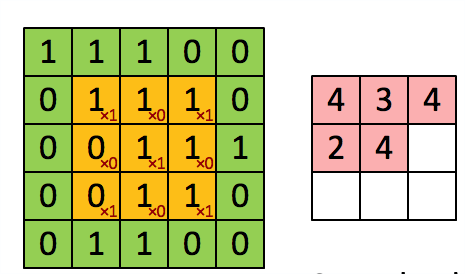
\includegraphics[width=0.4\textwidth]{convolution}
    \caption{Konvolúcie v CNN, zelená matica je vstupný obrázok a žltá matic je filter(vľavo), extrahované príznaky(vpravo) \cite{odkaz:CNNArticle}.}
    \label{pic:Convolution}
\end{figure}

Veľkosť aktivačnej mapy je možné nastaviť pomocou 3 parametrov.
\begin{enumerate}
    \item[$\bullet$] \textbf{Hĺbka} [eng. Depth] - veľkosť hĺbky zodpovedá počtu použitých filtrov v konvolučnej vrstve siete.
    \item[$\bullet$] \textbf{Krok} [eng. Stride] - počet pixelov o ktorý sa filter posúva počas výpočtu aktivačnej mapy.
    Použitím väčších skokou bude výsledna aktivačná mapa menšia.
    \item[$\bullet$] \textbf{Nulový doplnok} [eng. Zero-padding] - občas je vhodné vložiť nulový doplnok okolo vstupného obrázku.
    Tento spôsob nám umožnuje ovládať veľkosť výstupej aktivačnej mapy.
\end{enumerate}


\subsubsection{Zlučovanie}
Zlučovanie [eng. Pooling] je další krok ktorý sa vykonáva v CNN, tento krok je vykonaný v Pooling vrstvách siete.
Jeho funkciou je znižovanie dimenzionality vstupnej aktivačnej mapy ale so snahou zachovať dôležitú informáciu ktorá táto mapa obsahuje.
Existuje niekoľko rôznych typov zlučovania npr. maximum, priemer alebo suma.

Pre tento krok je potrebné definovať veľkost okna (npr. 2x2 pixely) a krok o ktorý sa bude toto okno posúvať.
V prípade typu Max Pooling s veľkosťou filtra 2x2 sa zoberú 4 hodnoty z aktivačnej mapy a vyberie sa z nich maximálna, podobným spôsobom
    fungujú aj ostatné typy zlučovania, ale výsledna hodnota je npr. priemer alebo suma týchto 4 hodnôt.
V praxi sa ukázalo že najvýhodnejší je výber maxima \cite{odkaz:CNNArticle}.
\begin{figure}[H]
    \centering
    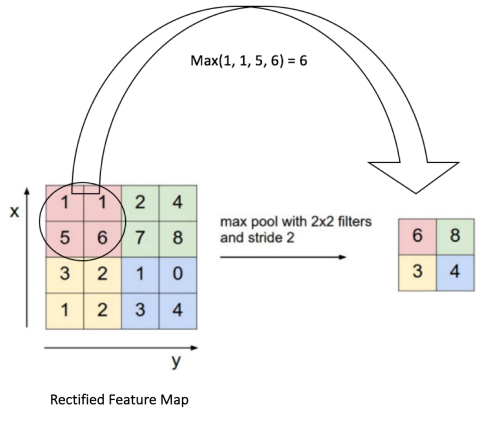
\includegraphics[width=0.6\textwidth]{pooling_original}
    \caption{Príklad použitia Max Pooling s filtrom 2x2 a krokom 2 \cite{odkaz:CNNArticle}.}
    \label{pic:Convolution}
\end{figure}


\subsubsection{Architektúra}
CNN využívajú skutočnosti, že vstup pozostáva z obrázkov.
Na rozdiel od obyčajnej neurónovej siete majú vrstvy CNN neuróny usporiadané v troch rozmeroch: šírka, výška, hĺbka [eng. width, height, depth].
Hĺbka odkazuje na 3.dimenziu aktivačného zväzku [eng. activation volume], nie na celkovú hĺbku neurónovej siete.
Neuróny vo vrtsve budú prepojené iba k malej oblasti vrstvy pred ňou, namiesto plného prepojenia \cite{odkaz:CNNArchitecture}.

Pre stavbu CNN sa využívajú 3 základne typy vrstiev a 1 podporná vrstva.
\begin{enumerate}
    \item[$\bullet$] \textbf{Convolutional layer} - konvolučná vrstva je hlavný stavebný blok CNN, ktorá vykonáva väčšinu výpočtov.
    Parametre tejto vrstvy pozostávajú zo súboru filtrov, ktoré sa dokážu učiť.
    Takto naučené filtre sa aktivujú keď uvidia určitý typ vizuálneho prvku, napr. hranu určitej orientácie alebo škvrnu určitej farby a pod..
    \item[$\bullet$] \textbf{Pooling layer} - táto vrstva je obvykle vkladaná ako spojenie medzi dvoma konvolučnímy vrstvami.
    Jej funkciou je postupné znižovanie priestorovej veľkosti reprezentovaného vstupu, pre zníženie množstva parametrov a výpočtov v sieti, a teda aj kontroly pretrénovania.
    \item[$\bullet$] \textbf{Fully-Connected layer} - rovnako ako v obvyklých neurónových sietach, je to vrstva kde všetky neuróny sú prepojené s predchádzajucou vrstvou.
    \item[$\bullet$] \textbf{Dropout layer} - cieľom tejto vrstvy je prevencia k pretrenovaniu siete, podľa nastavenia sa určité percento neurónov ktoré sa počas trénovanie zahadzuje.
    Táto vrstva tlačí neúronovú sieť k tomu aby sa učila na komplexnejších príznakoch, implementovaním tejto vrstvy do siete sa približne zdvojnásoby počet interácií trénovania.
    Avšak trénovaci čas pre každú iteráciu je kratší.
\end{enumerate}

\begin{figure}[H]
	\centering
	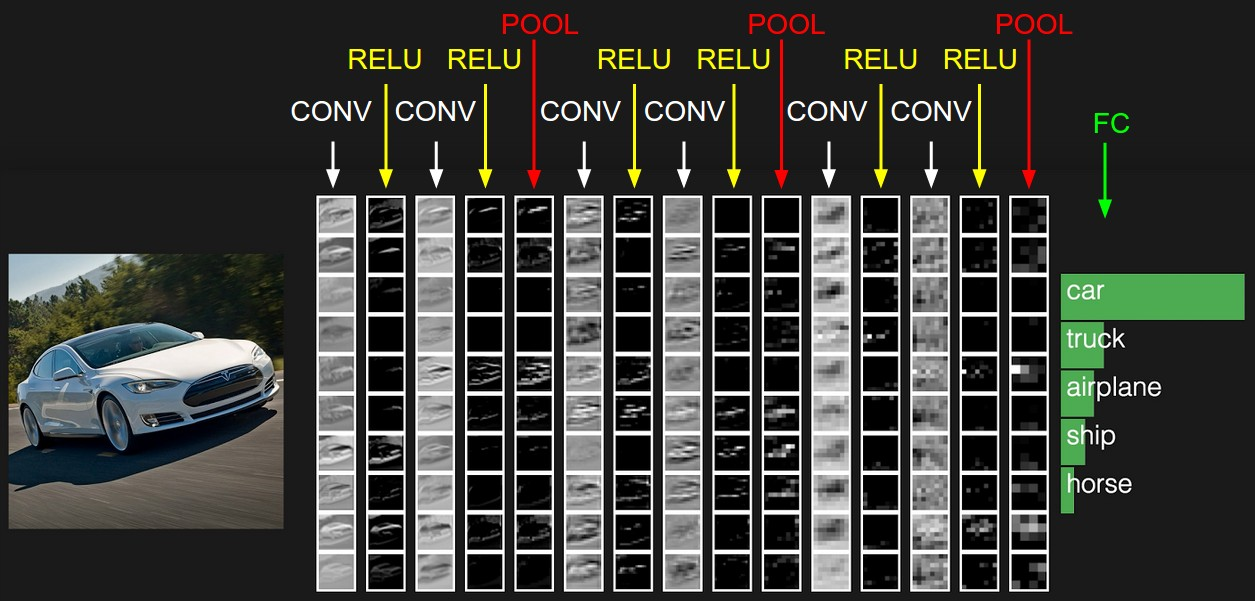
\includegraphics[width=1\textwidth]{convnet}
	\caption{Príklad architektúry konvolučnej neurónovej siete \cite{odkaz:CNNArchitecture}.}
	\label{pic:CNNExample}
\end{figure}

\subsection{Populárne architektúry}
\label{subsec:popularCNN}
Kedže konvolučné neurónove siete už existujú niekoľko rokov a komunita sa snaží o ich neustále zlepšovanie, tak sú organizované
    celosvetové súťaže na ktorých sa niekedy objaví architektúra siete ktorá dosahuje veľmi dobré výsledky a tak je možné ju použiť ako odporúčania a
    vychádzať z nej pri tvorbe vlastnej architektúry.

\textbf{AlexNet} (2012) je jedna z prvých hlbokých CNN. Táto sieť dala základ pre stavbu budúcich architektúr, zároveň bola použitá
    pre výhru v súťaži 2012 ILSVRC (ImageNet Large-Scale Visual Recognition Challenge).
V porovnaní s modernými architekturámi bola táto veľmi jednoduchá, tvorilo ju 5 konvolučných vrstiev, pooling vrstviev, dropout vrstiev a 3 plne prepojených vrstiev.
Siet bola použitá pre klasifikáciu objektov do 1000 kategórií.
Výchadzala z niekoľkých hlavných princípov \cite{odkaz:PopularCNN}:
\begin{enumerate}
    \item[$\bullet$] bola trénovaná na ImageNet\footnote{\url{http://www.image-net.org/}} databázovej sade, ktorá obsahuje cez 15 miliónov obrázkov vo viac ako 22000 kategóriách.
    \item[$\bullet$] Použila ReLU nelineárnu aktivačnú funkciu (objavil sa krátší čas trénovania, kedže výpočet ReLU je niekoľko krát rýchlejši ako oproti v tej dobe bežné používanej Tanh).
    \item[$\bullet$] Bola použítá technika augmentácie dát, ktorá pozostávala z rôznych transformácií obrázkov ako npr. horizontálny odraz.
    \item[$\bullet$] Implementovala Dropout vrstvy pre zníženie problému spojeným s pretrénovaním neúronovej siete.
    \item[$\bullet$] Trénovanie prebiehalo na dvoch GTX 580 grafických kartách, počas 5 až 6 dní.
\end{enumerate}

\textbf{VGG Net} (2014) je možné nájsť v niekoľkých variáciach, ako VGG16 alebo VGG19, čislo v názve udáva súčet konvolučným a plne prepojených vrstiev.
Veľkosti filtrov v konvolučným vrstvách sú o rozmeroch 3x3 oproti AlexNet kde ich veľkosť bola 11x11.
Avšak základna myšlienka tejto architektúry je v hĺbke a jednoduchosti, kedže zakladá na veľkom množstve konvolučným vrstiev z čoho vyplíva
    veľke množstvo filtrov a tým pádom zväčšuje svoj výstup do hĺbky.
Aj keď táto architektúra nebola výťaznou v roku 2014 na ILSVRC, ukázala základnu myšlienku že sieť môže byť jednoduchá ale musí byť hlboká \cite{odkaz:PopularCNN}.

\begin{figure}[H]
    \centering
    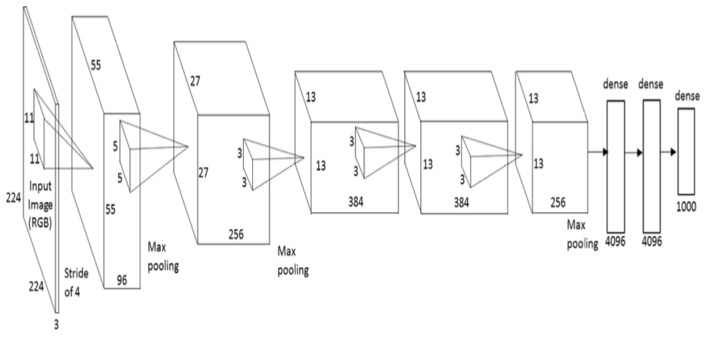
\includegraphics[width=0.8\textwidth]{alexnet}
    \qquad
    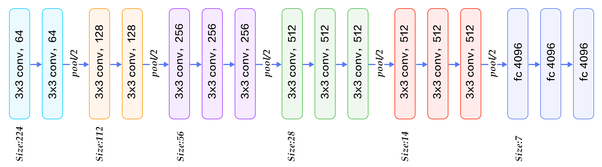
\includegraphics[width=0.8\textwidth]{vgg}
    \caption{Porovnanie architektúr AlexNet(hore) \cite{odkaz:AlexNet} a VGG16(dole) \cite{odkaz:VGG16}.}
    \label{pic:PopularCNN}
\end{figure}



\section{Nástroje pre tvorbu klasfikátorov a neurónových sieti}
\label{sec:frameworks}
V oblasti klasifikácie či už pomocou klasických prístupov alebo pomocou neurónových sieti, existuje množstvo nástrojov
    ktoré implementujú tieto techniky a sú voľné dostupné na použitie.
Technické giganty ako Google, Amazon, Facebook alebo Microsoft sú firmy ktoré vkladajú veľké investície do tejto oblasti.
Vedú buď svoj vlastný vývoj alebo získavajú/podporujú niektroé existujúce riešenia.
Kedže existuje veľke množstvo týchto nástrojov, tak v kapitole budú spomenuté iba niektoré, ktoré sa radia medzi najpopulárnejšie \cite{odkaz:FrameworkComparison}.

\subsubsection{Theano}

Theano je jeden z prvých nástrojov, vytvoril ho Yoshua Bengio spolu s výskumným tímom na University of Montreal v roku 2007.
Bol prvy široko používaný nástroj pre strojove učenie.
Theano je Python knižnica, extrémne rýchla a výkonná ale kritizovaná za to, že je nízko urovnovím nástrojom.
Tím ktorý stojí za touto knižnicou oznámil v roku 2017 že po vydaní poslednej verzie v roku 2018 už vývoj nebude pokračovať \cite{odkaz:FrameworkComparison}.

\subsubsection{TensorFlow}

TensorFlow je softvérová knižnica s otvoreným zdrojovým kódom[eng. open source library] pre numerické výpočty pomocou dátových vývojových diagramov[eng. data flow graphs].
Uzly v grafe reprezentujú matematické operácie, zatiaľ čo hrany grafu reprezentujú multidimenzionálne dátové polia (tensors), ktoré medzi sebou kominukujú.
Flexibilná architektúra umožňuje nasadenie na viacerých CPU alebo GPU, serveroch alebo aj mobilných zariadeniach.
TensorFlow bol pôvodne vyvinutý na účely výskumu strojového učenia a výskumu hlbokých neurónových sieti \cite{odkaz:TensorFlow}.

Aktuálne je TensorFlow najviac používaný systém pre trénovanie hlbokých neurónových sieti.
Stojí za ním veľká komunita technických firiem, odborníkov a technologický nadšenci z celého sveta, aj keď bola kritizovaná za jej prílišnu komplexnosť.
Ďalšou bežnou kritikou je, že podľa mnohých odborníkov je oveľa pomalšia v porovnaní s inými knižnicami \cite{odkaz:FrameworkComparison}.

\subsubsection{Keras}

Kedže vysoká všeobecnosť knižice TensorFlow pre jej širokú aplikáciu, robí jej použitie pre tvorbu neurónových sieti komplikovanejšiu.
Keras sa v tomto smere snaží využívať TensorFlow ako svoj backend a tvorbu neurónových sieti zjednodušiť.
Za jeho backend je možné použiť aj CNTK alebo Theano.
Táto implementácia knižnice Keras robí experimentovanie s neurónovými sietami jednoduchšie a rýchlejšie.
Aj keď sa snaží implementáciu zjednodušiť, stále si zachováva modularitu a preto je možné dostatočne dobre modely neurónových sieti upravovať a prisposobovať pre riešienie rôznych problémov \cite{odkaz:Keras}.

\subsubsection{PyTorch a Torch}

PyTorch je python implementácia nástroja Torch ktorý bol vydaní spoločnosťou Facebook v roku 2017.
Používa dynamické výpočtové grafy [eng. dynamic computational graphs], ktoré významne prispievajú k analýze neštrukturovaných údajov.
PyTorch si upravil alokátor GPU, ktorý umožnuje aby modely neurónových sieti boli viac pamäťovo efektívne.
Niektoré z hlavných nevýhod sú, že nástroj je stále v porovnateľne novej beta verzíí a nemá dostatočné veľkú podporu komunity \cite{odkaz:FrameworkComparison}.

\subsubsection{Caffe a Caffe2}

Caffe je dalši z nástrojov pre tvorbu neurónových sieti, avšak jeho použitie je priamo mierené pre spracovanie obrazu a nie na iné aplikácie
    ako spracovanie textu alebo zvuku \cite{odkaz:FrameworkComparison2}.
Za pritiotu si dáva rýchlosť a modularitu. Bol vyvinutý Berkley Artificial Intelligence Research.
Pre veľku popularitu Caffe sa Facebook rozhodol vydať Caffe2 v roku 2017.
Kde Caffe2 ponúka užívateľovi použiť predtrénované modely pre rýchlu tvorbu demo aplikácií \cite{odkaz:FrameworkComparison}.

\subsubsection{Scikit-learn a Scikit-image}

Scikit-learn je vysoko úrovňova knižnica navrhnutá pre algoritmy storjového učenia pod dozorom [eng. supervised learning] alebo bez dozoru [eng. unsupervised learning].
Ako jedna zo zložiek vedeckého ekosystému jazyka Python, je postavená na knižniciach NumPy a SciPy, kde každá z nich je zodpovedná za úlohy z vedeckej oblasti spracovania dát na nízkej úrovni.
Obsahuje množstvo algoritmov pre klasifikáciu, regresiu alebo zhlukovanie dát \cite{odkaz:FrameworkComparison3}.

Sciki-image je voľne dostupná knižnica ktorá obsahuje kolekciu algoritmov pre spracovanie obrázkov, určená pre SciPy.
Je písane v jazyku Python, knižnica je vývíjava SciPy komunitou \cite{prop:scikit-image}.



\section{Predspracovanie obrazu}

%http://scikit-image.org/docs/dev/auto\_examples/
% Normalizacia obrazu - github ten kurz c231n - 17150\_FULLTEXT.pdf (normalization)
%\subsection{Hogova transformacia}
% - F3-DP-2016-Erlebach-Jonas-Automaticka detekce pupily v obraze.pdf
%\subsection{Detekcia hran}
%- Sobelov filter - podľa knižky patri medzi najpopulárnejšie hranové filter. Urobiť z neho magnitúdu obrazu potom.

% Nieco na sposob ze, kedze riesenie bude obsahovat aj klasicke pristupy nie len riesenie s pouzitim
% neurovnovych sieti, je dolezite obrazky pred klasifikaciou vhodne upravit resp. extrahovat z obrazku vhodne priznaky na zaklade
% ktorych sa klasifikator bude ucit.

\subsubsection{Rovnomerný pomer strán}
Pre spracovanie obrázkov pomocou neurónových sieti je potrebné zabezpečiť, aby každý obrázok mal rovnakú veľkosť a rovnaký pomer strán.
Väčšina modelov neurónovej siete predpokladá štvorcový vstupný obraz \cite{odkaz:NNPreprocessing}.

\subsubsection{Priemerna štandartná odchylka vstupných údajov}
Je užitočné vytvoriť si tzv. ''stredný obraz'' získaný priemernými hodnotami pre každý pixel zo všetkých trénovacích dát.
Timto spôsobom je možné vytvoriť si základny prehľad o štruktúre vstupných dát.
Na základe toho môžeme potom do vstupným dát pridať rôzne dalšie variácie klasifikovaných objektov pre lepšie generalizovanie klasifikátora \cite{odkaz:NNPreprocessing}.

\subsubsection{Šedotónový obraz}
Ďalšou možnou technikou je vytvorenie šedotónového obrazu, kde všetky 3 zložky farby (RGB) zlúčime do jednej, šedotónovéj.
\begin{figure}[H]
	\centering
	
\includegraphics[width=0.4\textwidth]{grayscale}
	\caption{Prevod do šedotónového obrazu[eng. grayscaling]\cite{odkaz:NNPreprocessing}}
	\label{pic:GrayScaling}
\end{figure}

\subsubsection{Rožšírenie vstupných dát}
Ďalšou bežnou technickou predspracovanie dát je rožšírenie existujúceho súboru dát s rôznymi variáciami existujúcich obrázkov.
Tieto variácie môžu zahŕňať zväčšovanie, zmenšovanie, rotačné zmeny a iné transformácie obrázkov.
Tento postup znižuje šancu, že neurónová sieť rozpozná nežiadúce charakteristiky v množine vstupných dát \cite{odkaz:NNPreprocessing}.


\section{Zhrnutie kapitoly}


